\section{Esempi applicativi}
\subsection{Crollo di una diga}
Vediamo ora come utilizzare il codice in una applicazione reale: il crollo di una diga. Tale simulazione considera una situazione iniziale in cui la diga è chiusa; istantaneamente il muro di contenimento della diga crolla: la simulazione prende le mosse proprio da questo istante e si studia il comportamento del sistema nel tempo.

Il sistema è ben descritto dalle equazioni per le acque basse (o shallow waters) in due dimensioni:
\begin{equation} \label{eq:shallowwaters}
\begin{cases}
&\pdd{h}{t} + \pdd{(uh)}{x} + \pdd{(vh)}{x} = 0\\[1.5ex]
&\pdd{(uh)}{t} + \pdd{(u^2 h + gh^2/2)}{x} + \pdd{(uvh)}{y} = 0\\[1.5ex]
&\pdd{(vh)}{t} + \pdd{(uvh)}{x} + \pdd{(v^2 h +gh^2/2)}{y} = 0.
\end{cases}
\end{equation}
dove $h$ è il livello dell'acqua, $u$ e $v$ le componenti della velocità mentre $g$ è l'accelerazione di gravità.  

Definendo il vettore delle incognite $\textbf{q} = \left[ \begin{matrix} h & uh & vh \end{matrix} \right]^{\text{T}}$, è possibile riscrivere il sistema (\ref{eq:shallowwaters}) in forma vettoriale. In particolare, gli autovalori della matrice relativa al sistema sono:
\begin{equation*}
\left\{ \begin{aligned}
\lambda_{1} &= u n_x + v n_y \\[1.5ex]
\lambda_{2} &= u n_x + v n_y - c \left| \nn \right|\\[1.5ex]
\lambda_{2} &= u n_x + v n_y + c \left| \nn \right|
\end{aligned}  \right.
\end{equation*}
in cui $\nn$ è la normale (solitamente di norma unitaria) e $c = \sqrt{gh}$ è la velocità locale dell'onda.

All'istante zero il sistema ha velocità nulla: il fluido, a diga chiusa, è infatti fermo; l'altezza del fluido è 4.0 prima della barriera di contenimento e 1.0 dopo. Le condizioni al bordo sono differenti in base al lato che si considera: per sei lati, ovvero quelli che costituiscono la parte illesa della diga, condizioni al bordo riflettenti, mentre sui restanti lati si impongono condizioni assorbenti.

Nel problema viene considerato il dominio in Figura \ref{fig:dambreakdominio}, costruito in MatLab e già discretizzato in triangoli.
\begin{figure}[htb]
\centering
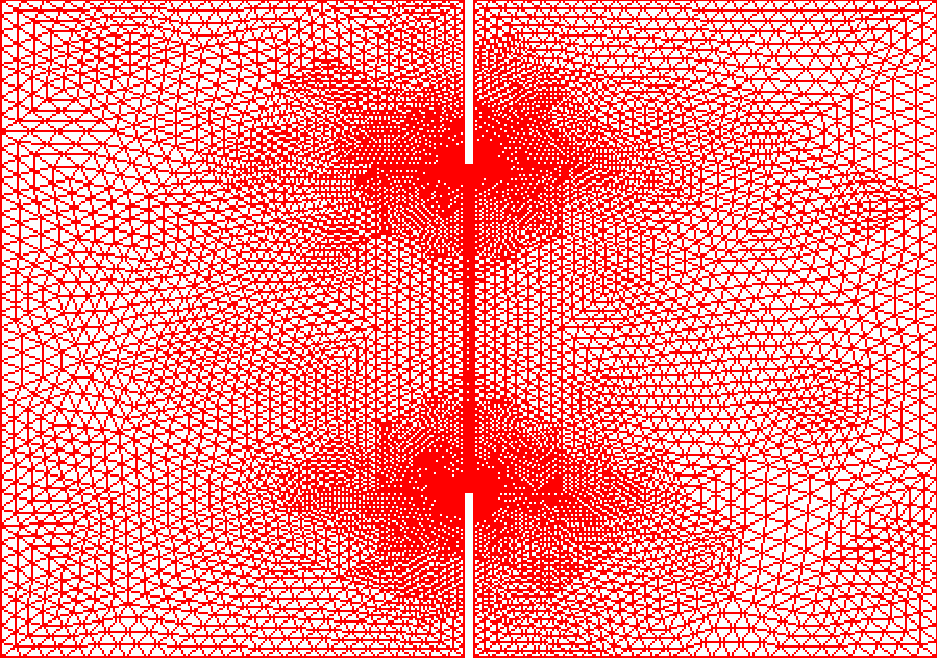
\includegraphics[width=8cm]{images/dambreak2dmesh.pdf}
\caption{Dominio di calcolo del problema del crollo della diga} \label{fig:dambreakdominio}
\end{figure}

Vediamo il programma. Si inizia includendo il modello (Shallow Waters), il flusso numerico di Lax-Friedrichs, il solutore a Volumi Finiti e il lettore della mesh.
\begin{lstlisting}[name=dambreak2d]
#include <models/shallowwater/shallowwater.hpp>
#include <solvers/fluxes/laxfriedrichs.hpp>
#include <solvers/finitevolume.hpp>
#include <mesh/io/meshreader.hpp>

#include <iostream>
#include <ctime>
#include <cmath>

using namespace std;
using namespace ConservationLaw2D;
\end{lstlisting}

A questo punto dobbiamo definire il solutore e tutto ciò che esso necessita. Da esso poi deriviamo la mesh, già particolareggiata per risolvere problemi con Volumi Finiti. Viene definito anche il tipo di soluzione, che sarà un vettore della giusta dimensione (grande tanto quante sono le variabili conservate, ossia 3). 
\begin{lstlisting}[name=dambreak2d]
typedef double real_t;
typedef Model::ShallowWater<real_t>              myModel;
typedef NumericalFlux::LaxFriedrichs<myModel>    myNumFlux;
typedef Solver::FiniteVolume<myModel,myNumFlux>  mySolver;
typedef mySolver::FVMesh                         myMesh;

// Tipo per la soluzione (vettore d-dim)
typedef myModel::SolType         SolType;
\end{lstlisting}
Definiamo ora le condizioni iniziali (nelle variabili primitive): a destra acqua alta, a sinistra acqua bassa.
\begin{lstlisting}[name=dambreak2d]
inline SolType init( size_t color, real_t x, real_t y ) {
    SolType sol = SolType::Zero();
    // rho, u, v
    sol[0] = ( x < 0 ) ? 4.0 : 1.0;
    sol[1] = 0.0;
    sol[2] = 0.0;
    return sol;
}
\end{lstlisting}
Analogamente per le condizioni al bordo (assorbenti nei lati esterni, di parete su quelle interne):
\begin{lstlisting}[name=dambreak2d]
inline SolType bc( SolType& wl, size_t color, real_t x, real_t y, real_t nx, real_t ny, real_t t ) {
    SolType wr = SolType::Zero();
    switch (color) {
        case 8:
        case 11:
        case 15:
        case 10:
        case 18:
        case 13:
            // Riflettente
            wr[0] = wl[0];
            wr[1] = (ny*ny-nx*nx)*wl[1] - 2*nx*ny*wl[2];
            wr[2] = - 2*nx*ny*wl[1] + (nx*nx-ny*ny)*wl[2];
            break;
        default:
           // Assorbente
           wr = wl;
           break;
    }
    return wr;
}
\end{lstlisting}
Come si osserva nella signature della funzione vengono passati lo stato a sinistra nelle variabili primitive wl, il colore del lato, le coordinate del punto medio, la normale e l'istante di tempo corrente.

Ora che ci sono tutti gli ingredienti si può inizializzare il problema:
\begin{lstlisting}[name=dambreak2d]
int main(int argc, char **argv) {
    // Parametri in ingresso
    bool gnuplot(false), interpolated(false);
    string meshfile;
    if ( argc < 2 ) {
        cout << "Usage: " << argv[0] << " [options] meshfile.msh" << endl;
        cout << "Options:" << endl;
        cout << "  --gnuplot\t\tGenerate plot and animation from gnuplot" << endl;
        cout << "  --interpolated\t\tInterpolate solution on vertices" << endl;
        exit(1);
    }
    for (int i=1; i<argc; ++i) {
        if (!strcmp(argv[i],"--gnuplot")) 
            gnuplot = true;
        else if (!strcmp(argv[i],"--interpolated"))
            interpolated = true;
        else
            meshfile = argv[i];
    }
    // Definisco il modello
    myModel model;
    // Definisco la mesh
    myMesh mesh;
    // Leggo la mesh
    Mesh::IO::MeshReader(mesh, meshfile);
    // Definisco il solutore per il mio modello
    mySolver solver(model, mesh);
    // Inizializzo alcuni parametri
    solver.setCFLmax(0.1);
    solver.setIC(init);
    solver.setBC(bc);
    solver.init();

    for (int i = 0; i < 1000; ++i) {
        std::cout << "== Timestep " << i << " == currtime: " << std::setw(8) << solver.getCurrTime();
        std::cout << ", dt = " << std::setw(8) << solver.getCurrDt() << std::endl;
        solver.timestep();
        if (i%50 == 0) solver.framegrab(i/50, gnuplot, interpolated);
    }
    return 0;
}
\end{lstlisting}
Nell'inizializzazione vengono automaticamente calcolate e salvate tutte le quantità geometriche fondamentali, per ottimizzare il solutore (linea 80). Nell'ultima parte invece viene fatto l'avanzamento in tempo vero e proprio.

L'esecuzione del programma è automatizzata attraverso lo script Perl postprocessing.py che richiede come argomento il file della mesh. 
Un output tipo è: 
\begin{verbatim}
>> Rimozione dati precedenti:   Fatto!
>> Simulazione:
=============================                      
Init Finite Volume Solver ...                      
=============================                      
== Timestep 0 == currtime:        0, dt = -0.0408514
== Timestep 1 == currtime: 8.61185e-05, dt = 8.61185e-05
== Timestep 2 == currtime: 0.000172237, dt = 8.61185e-05
[cut]
>> Genero frame 0:      Fatto!
>> Genero frame 1:      Fatto!
>> Genero frame 2:      Fatto!
[cut]
>> Genero animazione:   Fatto!
\end{verbatim}

Verrà rappresentata la soluzione in quattro istanti temporali successivi, in particolare si mostreranno l'andamento dell'altezza del fluido e il modulo della velocità (Figura \ref{fig:dambreak}).

\begin{figure}[htbp]
\centering
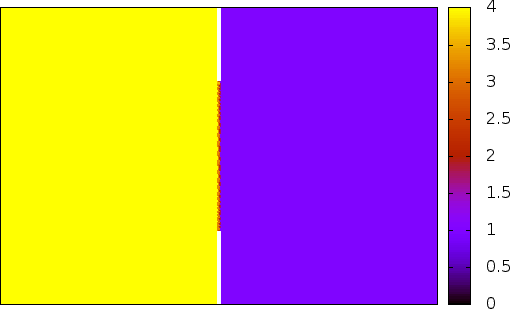
\includegraphics[width=0.4\textwidth]{images/DamBreak/height-solution0000.png} \hspace{0.2cm} 
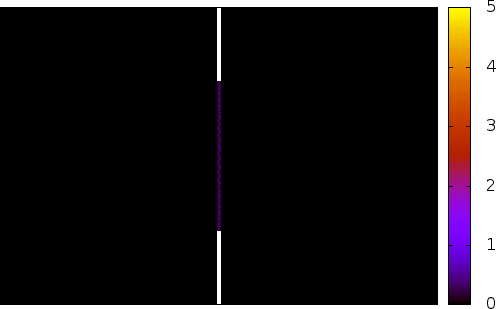
\includegraphics[width=0.4\textwidth]{images/DamBreak/velocity-solution0000.png} \\[0.5cm]
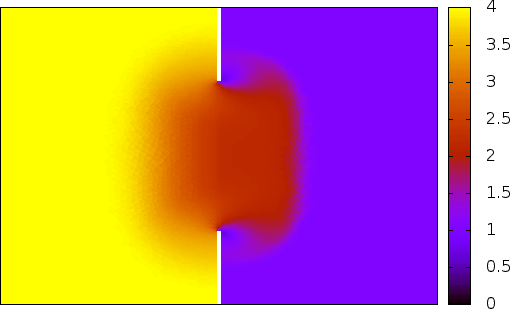
\includegraphics[width=0.4\textwidth]{images/DamBreak/height-solution0200.png} \hspace{0.2cm}
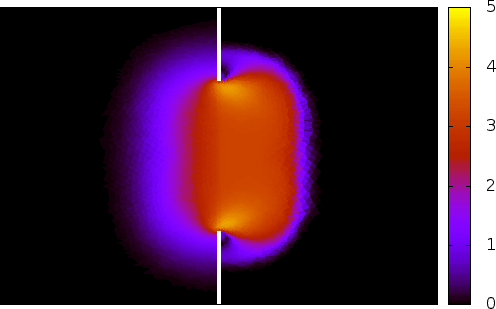
\includegraphics[width=0.4\textwidth]{images/DamBreak/velocity-solution0200.png}  \\[0.5cm] 
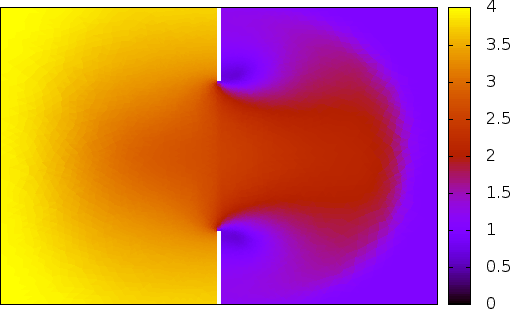
\includegraphics[width=0.4\textwidth]{images/DamBreak/height-solution0500.png}  \hspace{0.2cm}
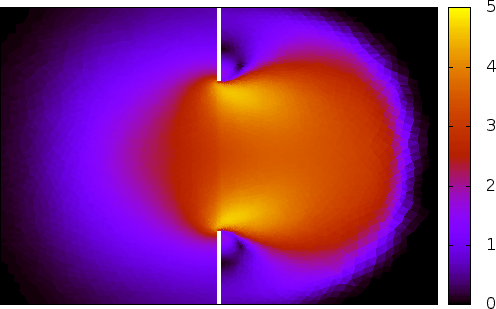
\includegraphics[width=0.4\textwidth]{images/DamBreak/velocity-solution0500.png}  \\[0.5cm]
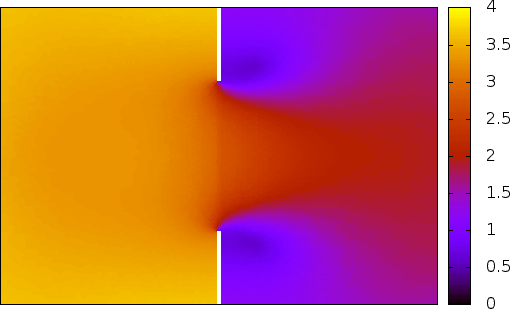
\includegraphics[width=0.4\textwidth]{images/DamBreak/height-solution0900.png}  \hspace{0.2cm}
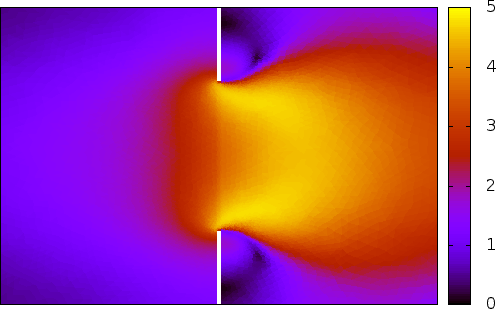
\includegraphics[width=0.4\textwidth]{images/DamBreak/velocity-solution0900.png}
\caption{Andamento dell'altezza (sinistra) e del modulo della velocità (destra) per il problema del crollo della diga con Lax-Friedrichs.}
\label{fig:dambreak}
\end{figure}

Questo test è molto semplice e lo schema ai Volumi Finiti riesce a cogliere con buona approssimazione tutti i fenomeni tipici del sistema. In particolare, notiamo che a valle della parete si generano zone di ricircolo e depressione che risultano ben definite. Inoltre, analizzando l'andamento del modulo di velocità, appare evidente l'aumento di velocità ai bordi dello sbocco e il successivo allargamento di vena a valle della diga.

Ovviamente la risoluzione è molto limitata dal fatto che stiamo utilizzando un metodo di ordine zero e un flusso numerico particolarmente dissipativo.

\subsection{Shock Bubble}
Presentiamo ora la soluzione ottenuta per il problema dello shock bubble, ovvero uno shock che investe una bolla di gas a densità minore. Lo schema numerico utilizzato è Roe con entropy fix. Viene mostrata la soluzione (rappresentata da densità e modulo della velocità) in quattro istanti temporali successivi (Figura \ref{fig:shockbubble}).
 
In particolare, il modello che regola il comportamneto del sistema è costituito dalle equazioni Eulero, che si ottiengono da quelle di Navier-Stokes considerando un fluido inviscido: si eliminano così tutti i contributi relativi alla viscosità e il sistema di equazioni si semplifica nel seguente modo:
\begin{equation} \label{eq:eulero}
\begin{cases}
&\pdd{\rho}{t} + \diverg \left(\rho \textbf{u}\right) = 0\\[1.5ex]
&\pdd{\left(\rho \textbf{u}\right)}{t} + \diverg \left(\rho \textbf{u} \otimes \textbf{u} + p \right) = \rho f^{V}\\[1.5ex]
&\pdd{\left(\rho e\right)}{t} + \diverg \left(\rho h \textbf{u} + \frac{1}{2} \rho |\textbf{u}|^{2} \textbf{u} \right) = \rho r + \rho f^{V} \textbf{u}
\end{cases}
\end{equation}
dove $\rho$ è la densità del fluido (non costante), $f^{V}$ sono le forze di volume agenti sul fluido, $e$ è l'energia specifica per unità di massa, $h$ è l'entalpia specifica e $r$ rappresenta un termine sorgente di calore per unità di massa e di tempo.  

Definendo il vettore delle incognite $\textbf{q} = \left[ \begin{matrix} \rho & \rho u & \rho v & \rho e \end{matrix} \right]^{\text{T}}$ il sistema \eqref{eq:eulero} si può scrivere in forma compatta in questo modo:
\begin{equation*}
\pdd{\textbf{q}}{t} + \pdd{\textbf{F}_{1}(\textbf{q})}{x} + \pdd{\textbf{F}_{2}(\textbf{q})}{y} = \textbf{S}(\textbf{q})
\end{equation*}
in cui $\textbf{S}(\textbf{q})$ rappresenta il vettore delle forzanti.
 
Tale relazione si può anche scrivere in forma quasi-lineare, il che permette di osservare nel nostro caso che si tratta di un problema \emph{iperbolico}: se si proietta questa equazione lungo una direzione $\nn$ si ottiene una matrice $\textbf{A}(\textbf{q};\nn)$ diagonalizzabile con tutti gli autovalori reali.
 
Nel caso di Eulero, gli autovalori della matrice $\textbf{A}(\textbf{q};\nn)$ sono infatti:
\begin{equation*}
\left\{ \begin{aligned}
\lambda_{1,4} &= \textbf{u} \cdot \nn \pm c \\[1.5ex]
\lambda_{2,3} &= \textbf{u} \cdot \nn
\end{aligned}  \right.
\end{equation*}
dove $c$ è la velocità locale del suono definita da $c = \sqrt{\partial{p}/\partial{\rho}}$. Possiamo osservare che l'autovalore $\lambda_{2,3}$ è degenere con molteplicità algebrica 2; le onde associate agli autovalori $\lambda_{1}$ e $\lambda_{4}$ sono onde sonore. Pertanto, alcune informazioni si propagano a velocità $\mathbf{u}\cdot\nn \pm c$ mentre altre sono trasportate dal flusso.

Per imporre le condizioni iniziali, il dominio di calcolo può essere diviso in tre zone: la prima zona è rappresentata dalla bolla, in cui $\rho = 0.1$, $p = 1$ , $u = v = 0 $; la seconda zona è quella a valle dello shock (bolla esclusa), in cui $\rho = 1$, $p = 1$ , $u = v = 0 $; mentre nella zona a monte della discontinuità si pone $p = 10$ mentre le altre grandezze si ricavano, essendo noti gli stati nelle altre zone. Le condizioni al bordo imposte sono tutte assorbenti.

\begin{figure}[htbp]
\centering
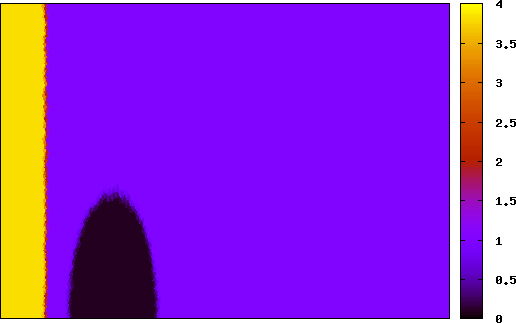
\includegraphics[width=0.4\textwidth]{images/ShockBubbleNew/height-solution0000bis.png} \hspace{0.2cm} 
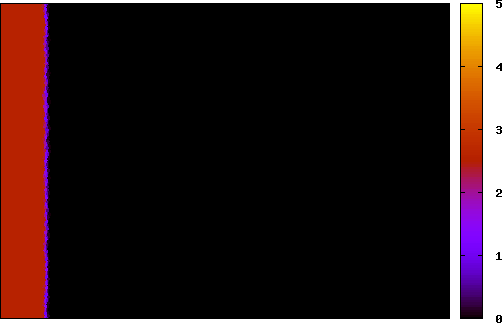
\includegraphics[width=0.4\textwidth]{images/ShockBubbleNew/velocity-solution0000bis.png} \\[0.5cm]
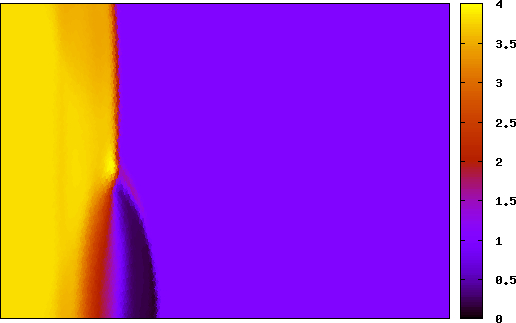
\includegraphics[width=0.4\textwidth]{images/ShockBubbleNew/height-solution0010bis.png} \hspace{0.2cm}
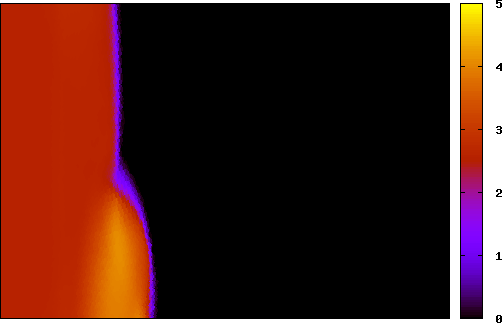
\includegraphics[width=0.4\textwidth]{images/ShockBubbleNew/velocity-solution0010bis.png}  \\[0.5cm] 
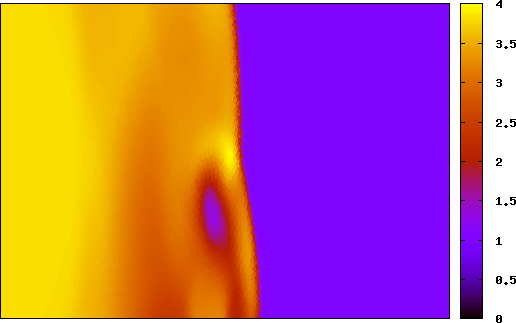
\includegraphics[width=0.4\textwidth]{images/ShockBubbleNew/height-solution0030bis.png}  \hspace{0.2cm}
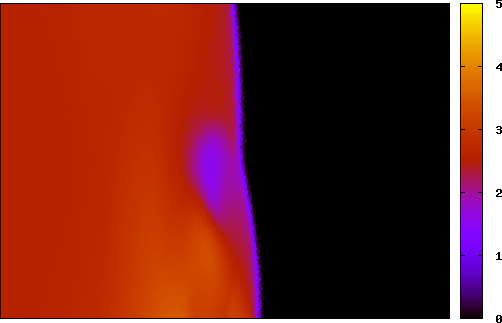
\includegraphics[width=0.4\textwidth]{images/ShockBubbleNew/velocity-solution0030bis.png}  \\[0.5cm]
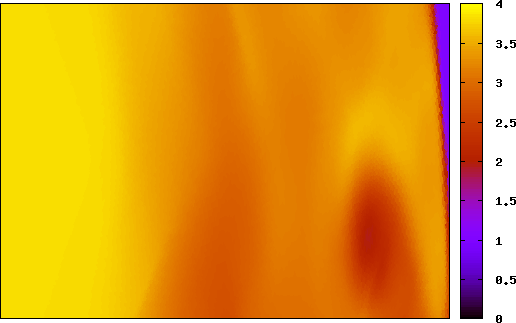
\includegraphics[width=0.4\textwidth]{images/ShockBubbleNew/height-solution0060bis.png}  \hspace{0.2cm}
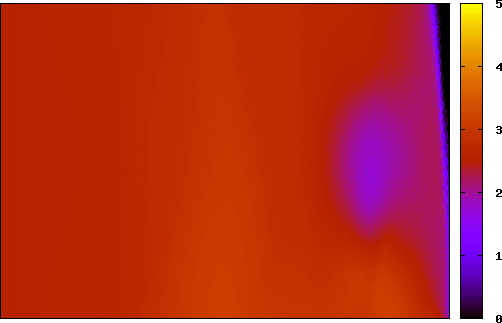
\includegraphics[width=0.4\textwidth]{images/ShockBubbleNew/velocity-solution0060bis.png}
\caption{Andamento della densità (sinistra) e del modulo della velocità (destra) per il problema shock bubble con Roe con entropy fix.}
\label{fig:shockbubble}
\end{figure}

La particolarità di questo esperimento (che alcuni ricercatori hanno anche eseguito realmente \cite{Williams1998307}) è che la bolla una volta investita dallo shock si avvolge su se stessa formando un toro: le immagini in Figura \ref{fig:shockbubble} devono essere pensate come una sezione di un volume a simmetria di rotazione.

Questo test numerico ci permette di osservare come il metodo dei Volumi Finiti necessiti di griglie molto fitte per ottenere risultati di buona qualità: in particolare, in questa simulazione si sono utilizzati circa 20000 triangoli, ma non sono stati sufficienti, infatti si sono persi molti dettagli interessanti dell'evoluzione del sistema (ad esempio, non sono definite molte zone di ricircolo e neanche le varie riflessioni che lo shock subisce).
